\documentclass[]{book}
\usepackage{lmodern}
\usepackage{amssymb,amsmath}
\usepackage{ifxetex,ifluatex}
\usepackage{fixltx2e} % provides \textsubscript
\ifnum 0\ifxetex 1\fi\ifluatex 1\fi=0 % if pdftex
  \usepackage[T1]{fontenc}
  \usepackage[utf8]{inputenc}
\else % if luatex or xelatex
  \ifxetex
    \usepackage{mathspec}
  \else
    \usepackage{fontspec}
  \fi
  \defaultfontfeatures{Ligatures=TeX,Scale=MatchLowercase}
\fi
% use upquote if available, for straight quotes in verbatim environments
\IfFileExists{upquote.sty}{\usepackage{upquote}}{}
% use microtype if available
\IfFileExists{microtype.sty}{%
\usepackage[]{microtype}
\UseMicrotypeSet[protrusion]{basicmath} % disable protrusion for tt fonts
}{}
\PassOptionsToPackage{hyphens}{url} % url is loaded by hyperref
\usepackage[unicode=true]{hyperref}
\hypersetup{
            pdftitle={Legal Probabilism and Its Limits},
            pdfauthor={Marcello Di Bello and Rafal Urbaniak},
            pdfborder={0 0 0},
            breaklinks=true}
\urlstyle{same}  % don't use monospace font for urls
\usepackage{color}
\usepackage{fancyvrb}
\newcommand{\VerbBar}{|}
\newcommand{\VERB}{\Verb[commandchars=\\\{\}]}
\DefineVerbatimEnvironment{Highlighting}{Verbatim}{commandchars=\\\{\}}
% Add ',fontsize=\small' for more characters per line
\usepackage{framed}
\definecolor{shadecolor}{RGB}{248,248,248}
\newenvironment{Shaded}{\begin{snugshade}}{\end{snugshade}}
\newcommand{\KeywordTok}[1]{\textcolor[rgb]{0.13,0.29,0.53}{\textbf{#1}}}
\newcommand{\DataTypeTok}[1]{\textcolor[rgb]{0.13,0.29,0.53}{#1}}
\newcommand{\DecValTok}[1]{\textcolor[rgb]{0.00,0.00,0.81}{#1}}
\newcommand{\BaseNTok}[1]{\textcolor[rgb]{0.00,0.00,0.81}{#1}}
\newcommand{\FloatTok}[1]{\textcolor[rgb]{0.00,0.00,0.81}{#1}}
\newcommand{\ConstantTok}[1]{\textcolor[rgb]{0.00,0.00,0.00}{#1}}
\newcommand{\CharTok}[1]{\textcolor[rgb]{0.31,0.60,0.02}{#1}}
\newcommand{\SpecialCharTok}[1]{\textcolor[rgb]{0.00,0.00,0.00}{#1}}
\newcommand{\StringTok}[1]{\textcolor[rgb]{0.31,0.60,0.02}{#1}}
\newcommand{\VerbatimStringTok}[1]{\textcolor[rgb]{0.31,0.60,0.02}{#1}}
\newcommand{\SpecialStringTok}[1]{\textcolor[rgb]{0.31,0.60,0.02}{#1}}
\newcommand{\ImportTok}[1]{#1}
\newcommand{\CommentTok}[1]{\textcolor[rgb]{0.56,0.35,0.01}{\textit{#1}}}
\newcommand{\DocumentationTok}[1]{\textcolor[rgb]{0.56,0.35,0.01}{\textbf{\textit{#1}}}}
\newcommand{\AnnotationTok}[1]{\textcolor[rgb]{0.56,0.35,0.01}{\textbf{\textit{#1}}}}
\newcommand{\CommentVarTok}[1]{\textcolor[rgb]{0.56,0.35,0.01}{\textbf{\textit{#1}}}}
\newcommand{\OtherTok}[1]{\textcolor[rgb]{0.56,0.35,0.01}{#1}}
\newcommand{\FunctionTok}[1]{\textcolor[rgb]{0.00,0.00,0.00}{#1}}
\newcommand{\VariableTok}[1]{\textcolor[rgb]{0.00,0.00,0.00}{#1}}
\newcommand{\ControlFlowTok}[1]{\textcolor[rgb]{0.13,0.29,0.53}{\textbf{#1}}}
\newcommand{\OperatorTok}[1]{\textcolor[rgb]{0.81,0.36,0.00}{\textbf{#1}}}
\newcommand{\BuiltInTok}[1]{#1}
\newcommand{\ExtensionTok}[1]{#1}
\newcommand{\PreprocessorTok}[1]{\textcolor[rgb]{0.56,0.35,0.01}{\textit{#1}}}
\newcommand{\AttributeTok}[1]{\textcolor[rgb]{0.77,0.63,0.00}{#1}}
\newcommand{\RegionMarkerTok}[1]{#1}
\newcommand{\InformationTok}[1]{\textcolor[rgb]{0.56,0.35,0.01}{\textbf{\textit{#1}}}}
\newcommand{\WarningTok}[1]{\textcolor[rgb]{0.56,0.35,0.01}{\textbf{\textit{#1}}}}
\newcommand{\AlertTok}[1]{\textcolor[rgb]{0.94,0.16,0.16}{#1}}
\newcommand{\ErrorTok}[1]{\textcolor[rgb]{0.64,0.00,0.00}{\textbf{#1}}}
\newcommand{\NormalTok}[1]{#1}
\usepackage{longtable,booktabs}
% Fix footnotes in tables (requires footnote package)
\IfFileExists{footnote.sty}{\usepackage{footnote}\makesavenoteenv{long table}}{}
\usepackage{graphicx,grffile}
\makeatletter
\def\maxwidth{\ifdim\Gin@nat@width>\linewidth\linewidth\else\Gin@nat@width\fi}
\def\maxheight{\ifdim\Gin@nat@height>\textheight\textheight\else\Gin@nat@height\fi}
\makeatother
% Scale images if necessary, so that they will not overflow the page
% margins by default, and it is still possible to overwrite the defaults
% using explicit options in \includegraphics[width, height, ...]{}
\setkeys{Gin}{width=\maxwidth,height=\maxheight,keepaspectratio}
\IfFileExists{parskip.sty}{%
\usepackage{parskip}
}{% else
\setlength{\parindent}{0pt}
\setlength{\parskip}{6pt plus 2pt minus 1pt}
}
\setlength{\emergencystretch}{3em}  % prevent overfull lines
\providecommand{\tightlist}{%
  \setlength{\itemsep}{0pt}\setlength{\parskip}{0pt}}
\setcounter{secnumdepth}{5}
% Redefines (sub)paragraphs to behave more like sections
\ifx\paragraph\undefined\else
\let\oldparagraph\paragraph
\renewcommand{\paragraph}[1]{\oldparagraph{#1}\mbox{}}
\fi
\ifx\subparagraph\undefined\else
\let\oldsubparagraph\subparagraph
\renewcommand{\subparagraph}[1]{\oldsubparagraph{#1}\mbox{}}
\fi

% set default figure placement to htbp
\makeatletter
\def\fps@figure{htbp}
\makeatother

\usepackage{todonotes}

\title{Legal Probabilism and Its Limits}
\author{Marcello Di Bello and Rafal Urbaniak}
\date{2021-05-05}

\begin{document}
\maketitle

{
\setcounter{tocdepth}{1}
\tableofcontents
}
\part{Legal probabilism and its foes}

\section*{Overview}

\chapter{The emergence of legal probabilism}

\section{Famous cases}

\section{Probabilistic evidence}

\section{Trial by mathematics}

\section{Some history}

This chapter will introduce legal probabilism and contain an account of
early\\
discussions of legal probabilism, how it came about, when, major
contributions, etc. I see essentially two moments in the history of
legal probabilism: the early days when probability theory was invented
(Bernoulli, Laplace, Condorcet, etc.), and then the second half of the
20th century with the emergence of the New Evidence Scholarship
(Lempert) and law and economics. But the history might be more
complicated.

\chapter{A skeptical perspective}

This chapter would discuss puzzles and hypothetical scenarios, mostly
the debate about naked statistical evidence. This is a discussion of the
most compelling objections that have been raised against legal
probabilism. Most of these objections trace back to Cohen, although
other pivotal players are Laurence Tribe and Ronald Allen. I think this
chapter could also have a historical flavor or perhaps it could be more
systematic. Not sure about the best presentation format.

\section{The difficulty about conjunction}

\section{The complexity objection}

\section{The problem of corroboration}

\section{The problem of artificial precision}

\section{Naked statistical evidence}\label{sec:naked}

\section{The problem of priors}

\section{The reference class problem}

\section{Non-probabilistic perspectives}

Remember the three-fold distinction.

\part{Evidence assessment}

\section*{Overview}

After the first part, the rest of the book will be a deep dive into what
probability theory can do for us when it is applied to trial
proceedings.

Instead of addressing the common objections upfront, the strategy of the
book would be to set the objections aside -- keep them on the back
burner as it were -- and return to them once we have a clearer sense of
legal probabilism and its limits.

\todo{We need to clearly set the limit of discussion of objections in the first part}

This part of the book is devoted to how probability theory can help---or
not help---in assessing trial evidence. I think it is important that we
start very simple and then we progressively get more complex.

\chapter{Bayes' Theorem and the usual fallacies}

This chapter shows how we can use probability theory and Bayes' theory
to spot common probabilistic fallacies, prosecutor's fallacy, base rate
fallacy, etc. This is the simple stuff.

I think this chapter should also show the limitation of this approach.
That is, we should make clear that these are probabilistic fallacies.
They are fallacies only insofar as the trier of facts aim to determine
the posterior probability of guilt. Which they might not.
\todo{careful here, some come up without explicit calculations}

The chapter will also be accompanied by case studies.

\section{Assuming independence}

\section{The prosecutor's fallacy}

\section{Base rate fallacy}

\section{Defense attorney's fallacy}

\section{Uniqueness fallacy}

\section{Case studies}

\subsection{Collins}

\subsection{Sally Clark}

\chapter{Complications and caveats}

\todo{not sure if this isn't too early}

Here we examine a number of complications that emerge from the simple
Bayes' theorem approach described in the earlier chapter. Here are some
of the common difficulties:

\begin{itemize}
 
 \item How do we determine the priors?
 
 \item More generally, how do we determine the numerical 
 values of any of the probabilities involved? 
 It might work for DNA matches, but what about non0numerical evidence 
 such as eyewitnesses? 
 
 \item How do we combine different pieces of evidence?  
 
 \item How we we formulate complex hypotheses, 
 say narratives, stories or explanations? 
 
 \item How do we take into account things 
 like the coherence of one's story or 
 the explanatory power of one's hypothesis?
 (evidence-to-hypothesis reasoning 
 versus hypothesis-to-evidence reasoning).
 
 \item Ronald Allen's objections 
 and Susan Haack's objections. 
 
 \end{itemize}

\section{Complex hypotheses and complex bodies of evidence}

\section{Source, activity and offense level hypotheses}

\section{Where do the numbers come from?}

\section{Modeling corroboration}

\section{Stories, explanations and coherence}

\chapter{Likelihood Ratios and Relevance}

Here we present likelihood ratios as a possible answer to some of the
complications. Pros and cons of this approach. It addresses the problems
of priors to some extent, but it leaves a lot of the other complications
essentially unresolved. The likelihood approach raises complication of
its own.

\section{Odds version of Bayes' theorem}

\section{Bayesian factor v. likelihood ratio}

\section{Choosing competing hypotheses}

\section{The two-stain problem}

\section{Case study: cold-hit DNA match evaluation}

\chapter{Bayesian Networks}

Here we present Bayesian networks as the best answer that legal
probabilists can offer. We illustrate Bayesian networks with examples
and show how they can answer some of the complications. We try to be as
honest as possible. We want to be a reliable and trustworthy source of
discussion, not partisan. We also discuss how Bayesian networks can help
address certain puzzles about relevance.

\section{Bayesian networks to the rescue}

\section{Legal evidence idioms}

\section{Scenario idioms}

\section{Modeling relevance}

\section{Case study: Sally Clark}

\todo{Do we really want to get into BNs for DNA evidence evaluation?}

\section{DNA evidence}

\todo{We already mention corroboration at two places, we should clean this up.}

\chapter{Corroboration}

Here we zoom into a particular topic. This should be a place to review
the literature on corroboration and for Rafal to present his own
probabilistic solution to the corroboration puzzle.

Use BNs in the exposition!

\section{Boole's formula and Cohen's challenge}

\section{Modeling substantial rise in case of agreement}

\section{Ekel\"of's corroboration measure and evidentiary mechanisms}

\section{General approach  with multiple false stories and multiple witnesses}

\chapter{Coherence}

Looks like coherence (cohesiveness and related ideas) plays an important
role in assessing evidence at trial. Here it would be place to review
the literature on coherence and for Rafal to preset his own
probabilistic solution to the coherence puzzle, emphasizing legal
applications.

\section{Existing probabilistic coherence measures}

\section{An array of counterexamples}

\section{Coherence of structured narrations 
with Bayesian networks}

\section{Application to legal cases}

\chapter{New legal probabilism}

\section{Desiderata}

Refer back to the three perspectives.

\section{A probabilistic framework for narrations}

\section{Probabilistic explications of the desiderata}

\section{Bayesian network implementation}

\todo{perhaps Allen, Haack \& Moss here? }

\begin{itemize}
\item
  The Dutch school and its challenges
\item
  Merging/aggregation/selection issues
\item
  Conditions on narration
\item
  Formal representation and programmatic deployment
\end{itemize}

\part{Trial Decisions}

\section*{Overview}

We turn from assessing evidence to trial decisions. The question is
this, when is the evidence strong enough to meet the governing burden of
proof?

\chapter{The functions of the proof standards}

\section{Conceptual desiderata}

\section{Protecting defendants}

(re Winship)

\section{Error reduction and error distribution/allocation}

(Laudan, Stein, Allen)

\section{Dispute resolution and public deference}

(Nesson)

\section{Justification and answerability}

(Duff)

\chapter{Standards of proof}

\section{Legal background}

\section{Probabilistic thresholds}

\section{Theoretical difficultiies}

\section{Likelihood approach}

\section{The difficulties perist}

\section{Bayesian networks and probabilistic standard of proof}

\chapter{Accuracy and the risk of error}

This chapter introduces different ways to think about the risk of error
at trial.

\section{Minimizing expected costs}

Thisreviews the literature that describes how expected utility can be
used to define rules for trial decisions.

\section{Minimizing expected errors}

\section{Expected v.\ actual errors}

\section{Competing accounts 
of the risk of error}

One dimension of the risk of error flows from the posterior
probabilities \(P(Guilt | Evidence)\). The other dimension flows from
the conditional probabilities \(P(Conviction | Innocence)\). This an
opportunity for Marcello to present the arguments in his Mind paper,
which however Rafal has criticized. So hopefully this chapter will be a
very balanced account of the topic!

\section{Bayesian networks and 
the risk of error}

\chapter{Fairness in trial decisions}

This chapter discusses how decisions can be fair and to what extent
probability theory can help us think about the fairness of decisions.
One important notion of fairness that probability theory can capture is
that of equal distribution of the risk of error. This draws on some of
Marcello's argument in the Ethics paper.

\todo{talk about incompatibility of definitions, Hedden's argument against measures of fairness etc.}

\section{Procedural v.\ substantive fairness}

\section{Competing measures of substantive fairness}

\section{Bayesian networks and fairnesss}

\part{Putting it all together}

\section*{Overview}

\chapter{Alternative accounts and legal probabilism}

There exist several theoretical alternatives to the probabilistic
interpretation of proof standards in the scholarly literature. Some
scholars, on empirical or normative grounds, resist the claim that the
point of gathering and assessing evidence at trial is solely to estimate
the probability of the defendant's civil or criminal liability.

\section{Baconian probability}

This is Cohen's stuff, also followed by Alex Stein. (Stein,
\protect\hyperlink{ref-stein2008}{2008}) argues that, in order to
warrant a verdict against the defendant, the evidence should have
withstood objections and counterarguments, not merely supporting a high
probability.

\section{Relative Plausibility}

(Pennington \& Hastie, \protect\hyperlink{ref-Pennington1991}{1991},
Pennington \& Hastie (\protect\hyperlink{ref-penn1993}{1993})) have
proposed the \textit{story model} according to which judges and jurors,
first make sense of the evidence by constructing stories of what
happened, and then select the best story on the basis of multiple
criteria, such as coherence, fit with the evidence and completeness.
Along similar lines, ({\textbf{???}}) argue that the version of the
facts that best explains the evidence should prevail in a court of law.
For a discussion of inference to the best explanation in legal
reasoning, see (Schwartz \& Sober,
\protect\hyperlink{ref-schwartz2019WhatRelativePlausibility}{2019},
Hastie
(\protect\hyperlink{ref-hastie2019CaseRelativePlausibilitya}{2019}), Ho
(\protect\hyperlink{ref-lai2019HowPlausibleRelative}{2019}), Dale A
Nance
(\protect\hyperlink{ref-nance2019LimitationsRelativePlausibility}{2019})).

\section{Arguments}

Another approach is due to (Gordon, Prakken, \& Walton,
\protect\hyperlink{ref-gordon2007}{2007}) and (Prakken \& Sartor,
\protect\hyperlink{ref-prakken2009}{2009}) who view the trial as a place
in which arguments and counterarguments confront one another. The party
that has the best arguments, all things considered, should prevail. On
this view, probability estimates can themselves be the target of
objections and counterarguments.

\section{Sensitivity}

\section{Normic Support}

Martin Smith approach.

\section{Justification/foundherentism}

(Ho, \protect\hyperlink{ref-ho2008philosophy}{2008}) and (Haack,
\protect\hyperlink{ref-Haack2014-HAAEMS}{2014}) hold that degrees of
epistemic warrant for a claim, which depend on multiple factors -- such
as the extent to which the evidence supports the claim and it is
comprehensive -- cannot be equated to probabilities.

\section{Completeness}

Discuss here Nance proposal. (Dale A. Nance,
\protect\hyperlink{ref-nance2016}{2016}) argues that the evidence on
which to base a trial decision should be reasonably complete---it should
be all the evidence that one would reasonably expect to see from a
conscientious investigation of the facts. A similar argument can be
found in (Davidson \& Pargetter,
\protect\hyperlink{ref-davidsonpargetter1987}{1987}). Arguably,
probability-based decision thresholds can accommodate these
considerations, for example, by lowering the probability of civil or
criminal liability whenever the body of evidence is one-sided or
incomplete (Kaye, \protect\hyperlink{ref-Kaye79gate}{1979}, Kaye
(\protect\hyperlink{ref-Kaye1986Do}{1986}), Friedman
(\protect\hyperlink{ref-friedman1996}{1996})). Another strategy is to
give a probability-based account of the notion of completeness of the
evidence and other seemingly non-probabilistic criteria
({\textbf{???}}).

\section{Relevant alternatives}

(Gardiner, \protect\hyperlink{ref-gardiner2019ppa}{2019}) argues that
standards of proof should rule out all error possibilities that are
relevant and these need not coincide with error possibilities that are
probable.

\section{Knowledge}

Some epistemologists argue that a probabilistic belief, no matter how
high, is not enough to warrant knowledge, and knowledge should be the
standard for trial verdicts.

\chapter{Conclusions}

I'd like this conclusion to be a very careful and nuanced discussion of
the good and bad things about legal probabilism. What difficulties can
in principle be overcome and what other difficulties are instead
inherent to legal probabilism and thus inescapable?

\chapter*{Preface}\label{preface}
\addcontentsline{toc}{chapter}{Preface}

testing again

\begin{align} 
  f\left(k\right) = \binom{n}{k} p^k\left(1-p\right)^{n-k}
  \label{eq:binom}
\end{align}

This is a citation (Diamond, \protect\hyperlink{ref-diamond90}{1990})
which uses keys from the bib file listed in the preamble.

Equation \eqref{eq:binom}\footnote{This is a footnote containing a double
  citation (Dahlman, \protect\hyperlink{ref-dahlmanNakedStat2020}{2020};
  Diamond, \protect\hyperlink{ref-diamond90}{1990}).}

Note that chapter files are found and compiled automatically, but the
file names have to contain chapter numbers first. For instance, we used
\texttt{01-intro.Rmd}, placed in the same folder. Observe how we
included r code inline.

\begin{Shaded}
\begin{Highlighting}[]
\KeywordTok{plot}\NormalTok{(cars)}
\end{Highlighting}
\end{Shaded}

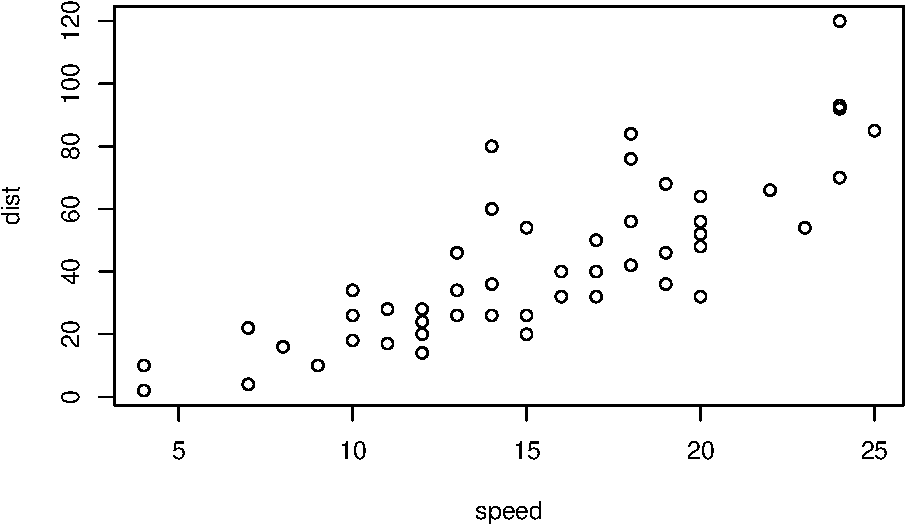
\includegraphics{_main_files/figure-latex/fig-margin-1.pdf}

\chapter{Introduction}\label{ch:intro}

You can label chapter and section titles using \texttt{\{\#label\}}
after them, e.g., we can reference Chapter \ref{ch:intro}. Let's use
chapter labels starting with ``ch:''.

Figures and tables with captions will be placed in \texttt{figure} and
\texttt{table} environments, respectively.

\begin{Shaded}
\begin{Highlighting}[]
\KeywordTok{par}\NormalTok{(}\DataTypeTok{mar =} \KeywordTok{c}\NormalTok{(}\DecValTok{4}\NormalTok{, }\DecValTok{4}\NormalTok{, }\FloatTok{.1}\NormalTok{, }\FloatTok{.1}\NormalTok{))}
\KeywordTok{plot}\NormalTok{(pressure, }\DataTypeTok{type =} \StringTok{'b'}\NormalTok{, }\DataTypeTok{pch =} \DecValTok{19}\NormalTok{)}
\end{Highlighting}
\end{Shaded}

\begin{figure}

{\centering 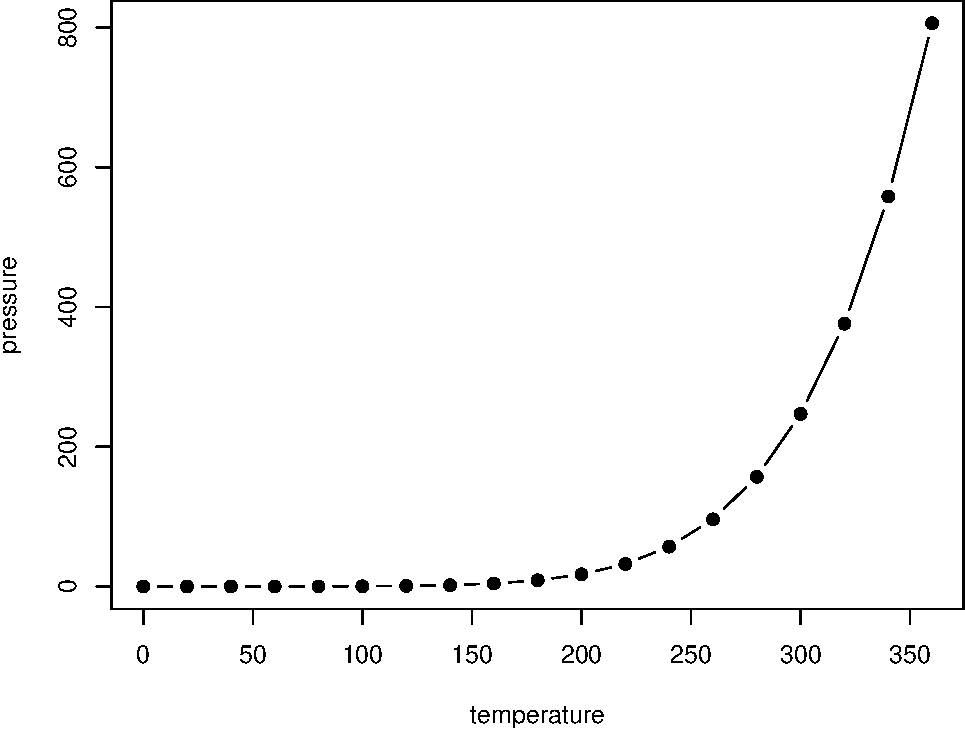
\includegraphics[width=0.8\linewidth]{_main_files/figure-latex/nice-fig-1} 

}

\caption{Here is a nice figure!}\label{fig:nice-fig}
\end{figure}

Reference a figure by its code chunk label with the \texttt{fig:}
prefix, e.g., see Figure \ref{fig:nice-fig}. Similarly, you can
reference tables generated from \texttt{knitr::kable()}, e.g., see Table
\ref{tab:nice-tab}.

\begin{Shaded}
\begin{Highlighting}[]
\NormalTok{knitr}\OperatorTok{::}\KeywordTok{kable}\NormalTok{(}
  \KeywordTok{head}\NormalTok{(iris, }\DecValTok{20}\NormalTok{), }\DataTypeTok{caption =} \StringTok{'Here is a nice table!'}\NormalTok{,}
  \DataTypeTok{booktabs =} \OtherTok{TRUE}
\NormalTok{)}
\end{Highlighting}
\end{Shaded}

\begin{table}

\caption{\label{tab:nice-tab}Here is a nice table!}
\centering
\begin{tabular}[t]{rrrrl}
\toprule
Sepal.Length & Sepal.Width & Petal.Length & Petal.Width & Species\\
\midrule
5.1 & 3.5 & 1.4 & 0.2 & setosa\\
4.9 & 3.0 & 1.4 & 0.2 & setosa\\
4.7 & 3.2 & 1.3 & 0.2 & setosa\\
4.6 & 3.1 & 1.5 & 0.2 & setosa\\
5.0 & 3.6 & 1.4 & 0.2 & setosa\\
\addlinespace
5.4 & 3.9 & 1.7 & 0.4 & setosa\\
4.6 & 3.4 & 1.4 & 0.3 & setosa\\
5.0 & 3.4 & 1.5 & 0.2 & setosa\\
4.4 & 2.9 & 1.4 & 0.2 & setosa\\
4.9 & 3.1 & 1.5 & 0.1 & setosa\\
\addlinespace
5.4 & 3.7 & 1.5 & 0.2 & setosa\\
4.8 & 3.4 & 1.6 & 0.2 & setosa\\
4.8 & 3.0 & 1.4 & 0.1 & setosa\\
4.3 & 3.0 & 1.1 & 0.1 & setosa\\
5.8 & 4.0 & 1.2 & 0.2 & setosa\\
\addlinespace
5.7 & 4.4 & 1.5 & 0.4 & setosa\\
5.4 & 3.9 & 1.3 & 0.4 & setosa\\
5.1 & 3.5 & 1.4 & 0.3 & setosa\\
5.7 & 3.8 & 1.7 & 0.3 & setosa\\
5.1 & 3.8 & 1.5 & 0.3 & setosa\\
\bottomrule
\end{tabular}
\end{table}

\hypertarget{refs}{}
\hypertarget{ref-dahlmanNakedStat2020}{}
Dahlman, C. (2020). Naked statistical evidence and incentives for lawful
conduct. \emph{International Journal of Evidence and Proof},
\emph{24}(2), 162--179.

\hypertarget{ref-davidsonpargetter1987}{}
Davidson, B., \& Pargetter, R. (1987). Guilt beyond reasonable doubt.
\emph{Australasian Journal of Philosophy}, \emph{65}(2), 182--187.

\hypertarget{ref-diamond90}{}
Diamond, H. A. (1990). Reasonable doubt: To define, or not to define.
\emph{Columbia Law Review}, \emph{90}(6), 1716--1736.

\hypertarget{ref-friedman1996}{}
Friedman, R. D. (1996). Assessing evidence. \emph{Michigan Law Review},
\emph{94}, 1810--1838.

\hypertarget{ref-gardiner2019ppa}{}
Gardiner, G. (2019). The reasonable and the relevant: Legal standards of
proof. \emph{Philosophy and Public Affairs}, \emph{47}(3), 288--318.

\hypertarget{ref-gordon2007}{}
Gordon, T. F., Prakken, H., \& Walton, D. (2007). The Carneades model of
argument and burden of proof. \emph{Artificial Intelligence},
\emph{171}(10-15), 875--896.

\hypertarget{ref-Haack2014-HAAEMS}{}
Haack, S. (2014). \emph{Evidence matters: Science, proof, and truth in
the law}. Cambridge University Press.

\hypertarget{ref-hastie2019CaseRelativePlausibilitya}{}
Hastie, R. (2019). The case for relative plausibility theory: Promising,
but insufficient. \emph{The International Journal of Evidence \& Proof},
\emph{23}(1-2), 134--140.

\hypertarget{ref-ho2008philosophy}{}
Ho, H. L. (2008). \emph{A philosophy of evidence law: Justice in the
search for truth}. Oxford University Press.

\hypertarget{ref-lai2019HowPlausibleRelative}{}
Ho, H. L. (2019). How plausible is the relative plausibility theory of
proof? \emph{The International Journal of Evidence \& Proof},
\emph{23}(1-2), 191--197.

\hypertarget{ref-Kaye79gate}{}
Kaye, D. H. (1979). The paradox of the Gatecrasher and other stories.
\emph{The Arizona State Law Journal}, 101--110.

\hypertarget{ref-Kaye1986Do}{}
Kaye, D. H. (1986). Do we need a calculus of weight to understand proof
beyond a reasonable doubt? \emph{Boston University Law Review},
\emph{66}, 657--672.

\hypertarget{ref-nance2016}{}
Nance, D. A. (2016). \emph{The burdens of proof: Discriminatory power,
weight of evidence, and tenacity of belief}. Cambridge University Press.

\hypertarget{ref-nance2019LimitationsRelativePlausibility}{}
Nance, D. A. (2019). The limitations of relative plausibility theory.
\emph{The International Journal of Evidence \& Proof}, \emph{23}(1-2),
154--160.

\hypertarget{ref-Pennington1991}{}
Pennington, N., \& Hastie, R. (1991). A cognitive theory of juror
decision making: The story model. \emph{Cardozo Law Review}, \emph{13},
519--557.

\hypertarget{ref-penn1993}{}
Pennington, N., \& Hastie, R. (1993). Reasoning in explanation-based
decision making. \emph{Cognition}, \emph{49}, 123--163.

\hypertarget{ref-prakken2009}{}
Prakken, H., \& Sartor, G. (2009). A logical analysis of burdens of
proof. In H. Kaptein, H. Prakken, \& B. Verheij (Eds.), \emph{Legal
evidence and proof: Statistics, stories, logic} (pp. 223--253). Ashgate.

\hypertarget{ref-schwartz2019WhatRelativePlausibility}{}
Schwartz, D. S., \& Sober, E. (2019). What is relative plausibility?
\emph{The International Journal of Evidence \& Proof}, \emph{23}(1-2),
198--204.

\hypertarget{ref-stein2008}{}
Stein, A. (2008). The right to silence helps the innocent: A reseponse
to critics. \emph{Cardozo Law Review}, \emph{30}(3), 1115--1140.

\end{document}
